\documentclass[11pt,a4paper]{report}
\usepackage[utf8]{inputenc}
\usepackage[T1]{fontenc}
\usepackage{geometry}
\usepackage{graphicx}
\usepackage{xcolor}
\usepackage{tikz}
\usepackage{tabularx}
\usepackage{enumitem}
\usepackage{fancyhdr}
\usepackage{hyperref}

\geometry{margin=2.5cm}

% Define brand colours
\definecolor{primaryblue}{RGB}{0,82,155}
\definecolor{secondarygreen}{RGB}{0,128,67}
\definecolor{accentgold}{RGB}{255,181,0}
\definecolor{darkgrey}{RGB}{64,64,64}
\definecolor{lightgrey}{RGB}{245,245,245}

\pagestyle{fancy}
\fancyhf{}
\fancyhead[L]{\textcolor{primaryblue}{\textbf{Brand Identity Guidelines}}}
\fancyhead[R]{\textcolor{darkgrey}{AI Strategy Platform}}
\fancyfoot[C]{\thepage}

\begin{document}

\begin{titlepage}
\centering
\vspace*{2cm}

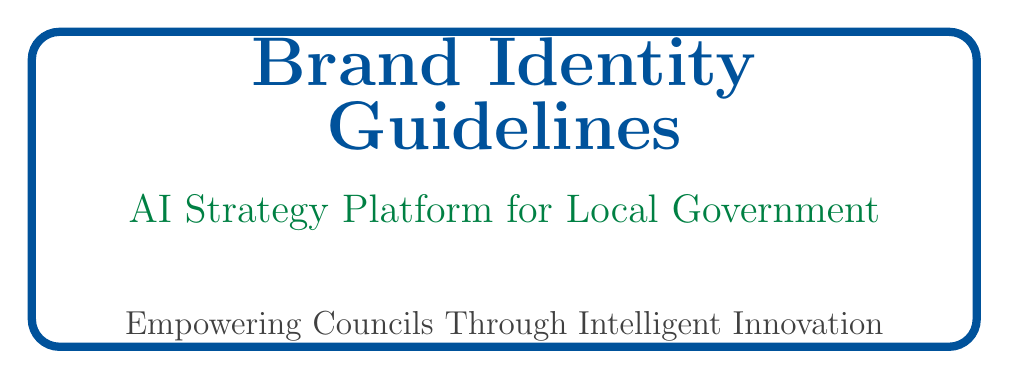
\begin{tikzpicture}
\node[draw=primaryblue, line width=3pt, minimum width=12cm, minimum height=4cm, rounded corners=10pt] (box) {};
\node at (box.center) {
    \begin{minipage}{10cm}
    \centering
    \textcolor{primaryblue}{\Huge\textbf{Brand Identity Guidelines}}\\[0.5cm]
    \textcolor{secondarygreen}{\Large AI Strategy Platform for Local Government}\\[1cm]
    \textcolor{darkgrey}{\large Empowering Councils Through Intelligent Innovation}
    \end{minipage}
};
\end{tikzpicture}

\vfill
\textcolor{darkgrey}{\large Version 1.0 | December 2024}
\end{titlepage}

\tableofcontents
\newpage

\chapter{Brand Foundation}

\section{Brand Purpose}
Our platform exists to democratise AI strategy development for UK local councils, transforming complex technological possibilities into actionable, ethical, and citizen-centric solutions.

\section{Brand Vision}
To become the trusted partner for every UK council in their AI transformation journey, creating a future where local government services are enhanced by intelligent, responsible AI implementation.

\section{Brand Mission}
We empower local government teams with intuitive AI strategy tools, expert guidance, and collaborative frameworks that translate cutting-edge technology into meaningful public service improvements.

\section{Brand Values}

\begin{itemize}[leftmargin=*]
\item \textbf{Accessibility}: Making AI strategy approachable for all council stakeholders
\item \textbf{Transparency}: Clear, open communication about AI capabilities and limitations
\item \textbf{Collaboration}: Fostering cross-council learning and best practice sharing
\item \textbf{Responsibility}: Prioritising ethical AI implementation and citizen privacy
\item \textbf{Innovation}: Continuous improvement driven by council feedback and needs
\item \textbf{Trust}: Building confidence through proven results and reliable support
\end{itemize}

\section{Brand Positioning Statement}
For UK local councils seeking to harness AI's potential, our platform is the comprehensive strategy solution that transforms technological complexity into clear, implementable plans. Unlike generic consultancy or technical platforms, we provide council-specific frameworks, collaborative tools, and ongoing support designed exclusively for local government needs.

\chapter{Brand Voice and Tone}

\section{Voice Characteristics}

\subsection{Professional yet Approachable}
\begin{itemize}
\item Use clear, jargon-free language
\item Explain technical concepts in accessible terms
\item Maintain authority without being intimidating
\end{itemize}

\subsection{Supportive and Empowering}
\begin{itemize}
\item Focus on possibilities and opportunities
\item Acknowledge challenges while providing solutions
\item Celebrate council achievements and progress
\end{itemize}

\subsection{Collaborative and Inclusive}
\begin{itemize}
\item Use "we" and "together" language
\item Emphasise partnership approach
\item Value diverse perspectives and experiences
\end{itemize}

\section{Tone Variations by Context}

\begin{tabularx}{\textwidth}{|l|X|X|}
\hline
\textbf{Context} & \textbf{Tone} & \textbf{Example} \\
\hline
Sales Materials & Confident, inspiring & "Transform your council's future with AI" \\
\hline
Technical Guides & Clear, instructive & "Follow these steps to implement your strategy" \\
\hline
Support Communications & Patient, helpful & "We're here to guide you through each stage" \\
\hline
Success Stories & Celebratory, proud & "Together, we've achieved remarkable results" \\
\hline
\end{tabularx}

\chapter{Visual Identity}

\section{Logo Design}

\begin{center}
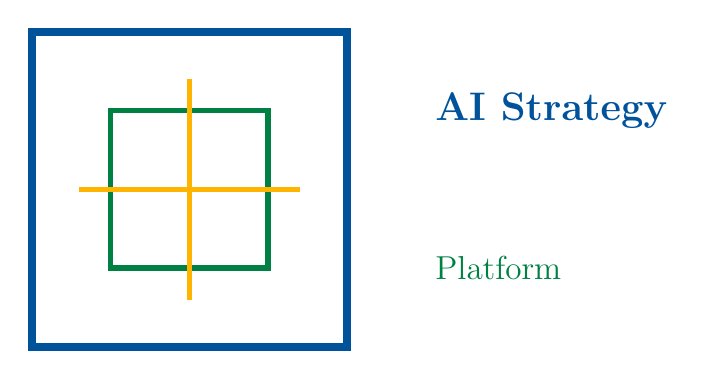
\begin{tikzpicture}[scale=2]
% Main logo mark
\draw[primaryblue, line width=3pt] (0,0) -- (2,0) -- (2,2) -- (0,2) -- cycle;
\draw[secondarygreen, line width=2pt] (0.5,0.5) -- (1.5,0.5) -- (1.5,1.5) -- (0.5,1.5) -- cycle;
\draw[accentgold, line width=2pt] (1,0.3) -- (1,1.7);
\draw[accentgold, line width=2pt] (0.3,1) -- (1.7,1);

% Text component
\node[right] at (2.5,1.5) {\Large\textbf{\textcolor{primaryblue}{AI Strategy}}};
\node[right] at (2.5,0.5) {\large\textcolor{secondarygreen}{Platform}};
\end{tikzpicture}
\end{center}

\subsection{Logo Usage Guidelines}
\begin{itemize}
\item Minimum clear space: 0.5x logo height on all sides
\item Minimum size: 25mm width for print, 120px for digital
\item Always maintain aspect ratio
\item Use on white or light backgrounds only
\end{itemize}

\section{Colour Palette}

\subsection{Primary Colours}
\begin{center}
\begin{tikzpicture}
\foreach \x/\col/\name/\rgb in {0/primaryblue/Primary Blue/0,82,155, 
                                 3/secondarygreen/Secondary Green/0,128,67,
                                 6/accentgold/Accent Gold/255,181,0} {
    \draw[fill=\col] (\x,0) rectangle (\x+2.5,2);
    \node[below] at (\x+1.25,-0.2) {\small\textbf{\name}};
    \node[below] at (\x+1.25,-0.6) {\tiny RGB: \rgb};
}
\end{tikzpicture}
\end{center}

\subsection{Supporting Colours}
\begin{center}
\begin{tikzpicture}
\foreach \x/\col/\name/\rgb in {0/darkgrey/Dark Grey/64,64,64,
                                 3/lightgrey/Light Grey/245,245,245} {
    \draw[fill=\col] (\x,0) rectangle (\x+2.5,2);
    \node[below] at (\x+1.25,-0.2) {\small\textbf{\name}};
    \node[below] at (\x+1.25,-0.6) {\tiny RGB: \rgb};
}
\end{tikzpicture}
\end{center}

\section{Typography}

\subsection{Primary Typeface}
\textbf{Headings}: Source Sans Pro Bold\\
\textit{Body Text}: Source Sans Pro Regular\\
\texttt{Technical Content}: Source Code Pro

\subsection{Typography Hierarchy}
\begin{itemize}
\item \textbf{H1}: 36pt, Primary Blue, Bold
\item \textbf{H2}: 28pt, Secondary Green, Bold
\item \textbf{H3}: 20pt, Dark Grey, Bold
\item \textbf{Body}: 12pt, Dark Grey, Regular
\item \textbf{Captions}: 10pt, Dark Grey, Italic
\end{itemize}

\chapter{Brand Architecture}

\section{Brand Hierarchy}

\begin{center}
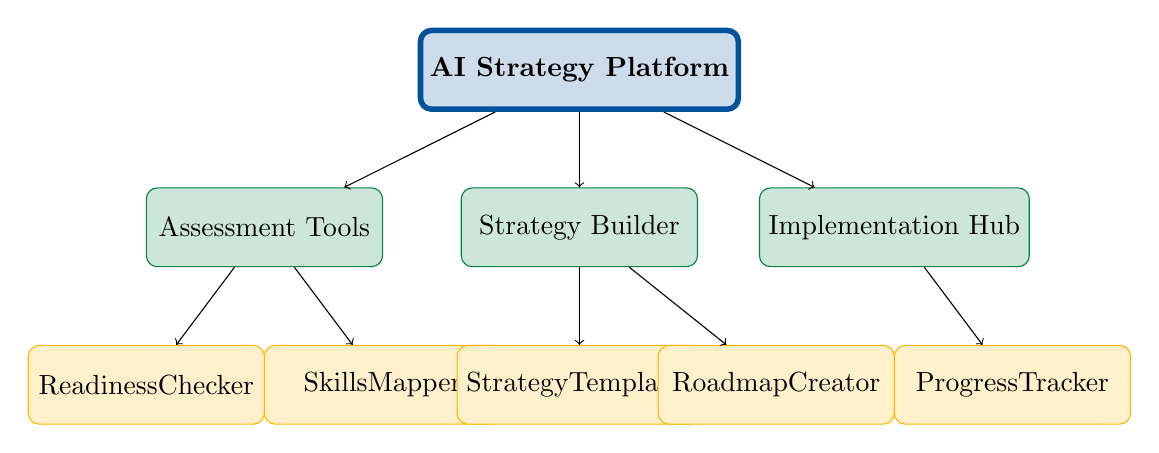
\begin{tikzpicture}[
    box/.style={draw, rounded corners, minimum width=3cm, minimum height=1cm, text centered},
    master/.style={box, fill=primaryblue!20, draw=primaryblue, line width=2pt},
    sub/.style={box, fill=secondarygreen!20, draw=secondarygreen},
    product/.style={box, fill=accentgold!20, draw=accentgold}
]

\node[master] (main) at (0,0) {\textbf{AI Strategy Platform}};

\node[sub] (assess) at (-4,-2) {Assessment Tools};
\node[sub] (develop) at (0,-2) {Strategy Builder};
\node[sub] (implement) at (4,-2) {Implementation Hub};

\node[product] (readiness) at (-5.5,-4) {Readiness\\Checker};
\node[product] (skills) at (-2.5,-4) {Skills\\Mapper};
\node[product] (templates) at (0,-4) {Strategy\\Templates};
\node[product] (roadmap) at (2.5,-4) {Roadmap\\Creator};
\node[product] (tracker) at (5.5,-4) {Progress\\Tracker};

\draw[->] (main) -- (assess);
\draw[->] (main) -- (develop);
\draw[->] (main) -- (implement);

\draw[->] (assess) -- (readiness);
\draw[->] (assess) -- (skills);
\draw[->] (develop) -- (templates);
\draw[->] (develop) -- (roadmap);
\draw[->] (implement) -- (tracker);

\end{tikzpicture}
\end{center}

\chapter{Application Guidelines}

\section{Digital Applications}

\subsection{Website Design Principles}
\begin{itemize}
\item Clean, uncluttered layouts with ample white space
\item Primary navigation using brand colours
\item Consistent use of typography hierarchy
\item Accessibility compliance (WCAG 2.1 AA minimum)
\item Mobile-first responsive design
\end{itemize}

\subsection{Email Templates}
\begin{itemize}
\item Header: Logo on white background
\item Body: Dark grey text on white
\item CTAs: Primary blue buttons with white text
\item Footer: Light grey background with contact details
\end{itemize}

\section{Print Applications}

\subsection{Business Cards}
\begin{center}
\begin{tikzpicture}[scale=0.8]
\draw[rounded corners=5pt] (0,0) rectangle (9,5);
\node at (1.5,3.5) {\includegraphics[width=2cm]{logo}};
\node[align=left] at (6,3.5) {\textbf{Name Surname}\\Title\\name@aiplatform.gov.uk\\07XXX XXXXXX};
\draw[primaryblue, line width=3pt] (0,0.5) -- (9,0.5);
\end{tikzpicture}
\end{center}

\subsection{Report Templates}
\begin{itemize}
\item Cover: Full-bleed primary blue with white logo
\item Headers: Secondary green with white text
\item Body: Dark grey on white background
\item Charts: Use brand colour palette
\end{itemize}

\chapter{Photography and Imagery}

\section{Photography Style}
\begin{itemize}
\item Authentic, candid shots of council teams collaborating
\item Bright, well-lit environments suggesting innovation
\item Diverse representation of council stakeholders
\item Technology integrated naturally into work settings
\item Focus on people using the platform, not just screens
\end{itemize}

\section{Iconography}
\begin{itemize}
\item Simple, line-based icons in brand colours
\item Consistent stroke width (2pt)
\item Rounded corners matching logo style
\item Clear metaphors avoiding technical complexity
\end{itemize}

\section{Illustration Guidelines}
\begin{itemize}
\item Flat design style with subtle gradients
\item Brand colour palette only
\item Abstract representations of AI concepts
\item Human-centric scenarios
\end{itemize}

\chapter{Brand in Action}

\section{Key Messages}

\subsection{Primary Message}
"Empowering councils to harness AI for better public services"

\subsection{Supporting Messages}
\begin{itemize}
\item "From complexity to clarity in AI strategy"
\item "Your partner in responsible AI transformation"
\item "Building tomorrow's councils, together"
\item "AI strategy made accessible, actionable, achievable"
\end{itemize}

\section{Elevator Pitch}
"We're the AI Strategy Platform designed exclusively for UK local councils. We transform the complexity of AI planning into clear, actionable strategies that improve public services while maintaining the highest standards of ethics and security. From initial assessment to full implementation, we guide councils through every step of their AI journey."

\section{Brand Personality Traits}
\begin{itemize}
\item \textbf{Knowledgeable}: Expert without being intimidating
\item \textbf{Supportive}: Always there when needed
\item \textbf{Progressive}: Forward-thinking yet practical
\item \textbf{Trustworthy}: Reliable and transparent
\item \textbf{Collaborative}: Working together for success
\end{itemize}

\end{document}